\documentclass[
10pt, % Main document font size
a4paper, % Paper type, use 'letterpaper' for US Letter paper
oneside, % One page layout (no page indentation)
%twoside, % Two page layout (page indentation for binding and different headers)
headinclude,footinclude, % Extra spacing for the header and footer
BCOR5mm, % Binding correction
]{scrartcl}

\usepackage{listings}
\usepackage{color}
%\usepackage{biblatex}

\definecolor{dkgreen}{rgb}{0,0.6,0}
\definecolor{gray}{rgb}{0.5,0.5,0.5}
\definecolor{mauve}{rgb}{0.58,0,0.82}

\lstset{frame=tb,
	language={Haskell},
	aboveskip=3mm,
	belowskip=3mm,
	showstringspaces=false,
	columns=flexible,
	basicstyle={\small\ttfamily},
	numbers=none,
	numberstyle=\tiny\color{gray},
	keywordstyle=\color{blue},
	commentstyle=\color{dkgreen},
	stringstyle=\color{mauve},
	breaklines=true,
	breakatwhitespace=true,
	tabsize=3
}

\usepackage{german}


%usepackage[utf8]{inputenc}
%\usepackage{geometry}
\usepackage[german,onelanguage,linesnumbered, ruled]{algorithm2e}
\SetAlFnt{\small}
\SetAlCapFnt{\large}
\SetAlCapNameFnt{\large}
%\usepackage{algpseudocode}


%%%%%%%%%%%%%%%%%%%%%%%%%%%%%%%%%%%%%%%%%
% Arsclassica Article
% Structure Specification File
%
% This file has been downloaded from:
% http://www.LaTeXTemplates.com
%
% Original author:
% Lorenzo Pantieri (http://www.lorenzopantieri.net) with extensive modifications by:
% Vel (vel@latextemplates.com)
%
% License:
% CC BY-NC-SA 3.0 (http://creativecommons.org/licenses/by-nc-sa/3.0/)
%
%%%%%%%%%%%%%%%%%%%%%%%%%%%%%%%%%%%%%%%%%

%----------------------------------------------------------------------------------------
%	REQUIRED PACKAGES
%----------------------------------------------------------------------------------------

\usepackage[
nochapters, % Turn off chapters since this is an article        
beramono, % Use the Bera Mono font for monospaced text (\texttt)
eulermath,% Use the Euler font for mathematics
pdfspacing, % Makes use of pdftex’ letter spacing capabilities via the microtype package
dottedtoc % Dotted lines leading to the page numbers in the table of contents
]{classicthesis} % The layout is based on the Classic Thesis style

\usepackage{arsclassica} % Modifies the Classic Thesis package

\usepackage[T1]{fontenc} % Use 8-bit encoding that has 256 glyphs

\usepackage[utf8]{inputenc} % Required for including letters with accents

\usepackage{graphicx} % Required for including images
\graphicspath{{Figures/}} % Set the default folder for images

\usepackage{enumitem} % Required for manipulating the whitespace between and within lists

\usepackage{lipsum} % Used for inserting dummy 'Lorem ipsum' text into the template

\usepackage{subfig} % Required for creating figures with multiple parts (subfigures)

\usepackage{amsmath,amssymb,amsthm} % For including math equations, theorems, symbols, etc

\usepackage{varioref} % More descriptive referencing

%----------------------------------------------------------------------------------------
%	THEOREM STYLES
%---------------------------------------------------------------------------------------

\theoremstyle{definition} % Define theorem styles here based on the definition style (used for definitions and examples)
\newtheorem{definition}{Definition}

\theoremstyle{plain} % Define theorem styles here based on the plain style (used for theorems, lemmas, propositions)
\newtheorem{theorem}{Theorem}

\theoremstyle{remark} % Define theorem styles here based on the remark style (used for remarks and notes)

%----------------------------------------------------------------------------------------
%	HYPERLINKS
%---------------------------------------------------------------------------------------

\hypersetup{
%draft, % Uncomment to remove all links (useful for printing in black and white)
colorlinks=true, breaklinks=true, bookmarks=true,bookmarksnumbered,
urlcolor=webbrown, linkcolor=RoyalBlue, citecolor=webgreen, % Link colors
pdftitle={}, % PDF title
pdfauthor={\textcopyright}, % PDF Author
pdfsubject={}, % PDF Subject
pdfkeywords={}, % PDF Keywords
pdfcreator={pdfLaTeX}, % PDF Creator
pdfproducer={LaTeX with hyperref and ClassicThesis} % PDF producer
} % Include the structure.tex file which specified the document structure and layout

\hyphenation{Fortran hy-phen-ation} % Specify custom hyphenation points in words with dashes where you would like hyphenation to occur, or alternatively, don't put any dashes in a word to stop hyphenation altogether

%----------------------------------------------------------------------------------------
%	TITLE AND AUTHOR(S)
%----------------------------------------------------------------------------------------

\title{\normalfont\spacedallcaps{Projektaufgabe AE}} % The article title

\subtitle{Remove Duplicates - Spotify playlist cleaner} % Uncomment to display a subtitle

\author{\spacedlowsmallcaps{Raphael Drechsler}} % The article author(s) - author affiliations need to be specified in the AUTHOR AFFILIATIONS block

\date{} % An optional date to appear under the author(s)

%----------------------------------------------------------------------------------------

\begin{document}

%----------------------------------------------------------------------------------------
%	HEADERS
%----------------------------------------------------------------------------------------

\renewcommand{\sectionmark}[1]{\markright{\spacedlowsmallcaps{#1}}} % The header for all pages (oneside) or for even pages (twoside)
%\renewcommand{\subsectionmark}[1]{\markright{\thesubsection~#1}} % Uncomment when using the twoside option - this modifies the header on odd pages
\lehead{\mbox{\llap{\small\thepage\kern1em\color{halfgray} \vline}\color{halfgray}\hspace{0.5em}\rightmark\hfil}} % The header style

\pagestyle{scrheadings} % Enable the headers specified in this block

%----------------------------------------------------------------------------------------
%	TABLE OF CONTENTS & LISTS OF FIGURES AND TABLES
%----------------------------------------------------------------------------------------

%\maketitle % Print the title/author/date block
{ \centering
{ \par}\
 \linebreak
\linebreak 
\linebreak
\linebreak
\linebreak
%\centering

\includegraphics[width=0.55\columnwidth]{htwLogo} 
\linebreak
\linebreak
\linebreak
\linebreak 
 % inline
{\fontsize{14}{16}\selectfont \center Fakultät Informatik, Mathematik und\\Naturwissenschaften\\Studiengang Informatik Master\par}\
 \linebreak
{\fontsize{18}{20}\selectfont \center \textbf{Projektarbeit zur Vorlesung Computermusik}\par}\
{\fontsize{20}{22}\selectfont \center \textbf{BrandtBrauerFrick.hs} \par}\
\linebreak
\linebreak
\linebreak
\linebreak 
\linebreak
\linebreak 
\linebreak 
{\fontsize{14}{16}\selectfont  \begin{tabular}{rl}
 	\textbf{Autoren:} & Nico Mehlhose, Raphael Drechsler\\ 
 	\textbf{Abgabedatum:} & 01.02.2019 \\ 
 \end{tabular}
\par}
\par}
\pagebreak
\setcounter{tocdepth}{2} % Set the depth of the table of contents to show sections and subsections only

%\tableofcontents % Print the table of contents
%\listoffigures % Print the list of figures
%\listoftables % Print the list of tables




%----------------------------------------------------------------------------------------

\newpage % Start the article content on the second page, remove this if you have a longer abstract that goes onto the second page

%----------------------------------------------------------------------------------------
%	INTRODUCTION
%----------------------------------------------------------------------------------------
\section{Abstract}\
\textit{Abschnitt bearbeitet von: Raphael Drechsler}\\

\noindent \textbf{BrandtBrauerFrick.hs}

\noindent Brandt Brauer Frick ist ein Techno-Projekt aus Berlin.
Die Basis des Projekts bilden Klänge aus dem Instrumentarium der
klassischen Musik, welche anfangs gesampelt, später in einem zehnköpfigen
Ensemble auch live vorgeführt wurden.\cite{Wiki}\\ 

\noindent Ziel des Projektes:\\
Die Umsetzung des Songs ''Pretend'' von Brandt Brauer Frick entweder in
Tidal oder Euterpea. Eine online verfügbare Live-Aufführung \cite{YT1} soll dabei als Referenz dienen. Bei der Umsetzung soll auch Wert auf die Nachbildung der echten Instrumente und deren teilweise Zweckentfremdung gelegt werden.\\

\noindent Herausforderungen:
\begin{itemize}
	\itemsep0em
	\item Evaluation ob Tidal\cite{Tidal} oder Euterpea\cite{Euterpea} genutzt werden soll:
	\item Untersuchung der Frage ob klassische Klänge am ehesten in Euterpea oder
	Tidal nutzbar sind. (Durch repetitiven Charakter des Liedes würde sich Tidal zur
	Live-Vorführung eignen)
	\item Analyse der einzelnen musikalischen Bausteine und deren Implementierung.
	\item Zusammenfügen der erarbeiteten Bausteine zu einer Performance.
\end{itemize}

\section{Umsetzung in Tidal oder Euterpea}\
\textit{Abschnitt bearbeitet von: Nico Mehlhose}\\

\noindent Dieses Thema soll sich um die Evaluation zwischen Tidal und Eutherpea handeln.\\
{\color{red}\textbf{TODO}}Was ist Tidal\cite{Tidal} (dazu SuperCollider\cite{SC} erklären) , was ist Euterpea\cite{Euterpea}?\\
Unsere Entscheidung Tidal zu nehmen beruht gewiss nicht auf einer zufälligen Entscheidung. In diese Entscheidung ist der Programmieraufwand, vorhandenen Informationen
und die Möglichkeit den Synthesizer zu erweitern.\\
Bei dem Programmieraufwand wird sehr schnell klar, dass durch das Lied \textit{Pretent} von BrandBrauerFrick Tidal besser geeignet ist als Euterpea. Der erste Gesichtspunkt
der betrachtet wurde ist die Repetetivität des Songs, welcher in Euterpea zwar auch umsetzbar ist aber in Tidal von Anfang an gegeben ist, da Tidal die Sounds immer in einem
Loop abspielt. Bei den vorhandenen Informationen stellt sich heraus, dass es keine Offiziellen Notenblätter für das Lied Onlinegibt, wodurch Euterpea etwas an Bedeutung verliert, da Euterpea für genaue Notenbestimmungen perfekt geeignet wäre. Da dieser Fakt aber nicht vorliegt, kann das selbe Maß an Genauigkeit auch mit Tidal erreicht werden.\\
Der letzte und für uns wichtigste Punkt war die Erweiterbarkeit der Sounds. Die Wichtigkeit darin besteht in der entfremdeten Benutzung der Musikinstrumente in dem Lied.
In Eutherpea haben wir nach einiger Recherche keinen weg gefunden Sounds hinzuzufügen um diese später zu verwenden. In Tidal allerdings existiert diese Möglichkeit mittels
des Befehl \textit{}. Mit diesem Befehl lässt sich ein Verzeichnis in Tidal integrieren.
%~dirt.loadSoundFiles("full/path/to/directory/*") noch in textit einfügen
\section{Eigenschaften des Stücks Pretend und dessen globale Struktur}\
\textit{Abschnitt bearbeitet von: Raphael Drechsler}\\

\noindent Die in der Live vorgeführte Version \cite{YT1} hat eine ungefähre Dauer von 7 Minuten, 15 Sekunden. Die Angabe erfolgt ungefähr, da die Aufnahme nicht mit dem ersten Takt beginnt\\
Per Gehör ließ sich feststellen, dass das Stück in der Tonart Gm steht.\\
Über ein BPM-Measuring-Tool \cite{tempo} wurde ein Tempo von 130bpm ermittelt. In Tidal wird somit der folgende Code zur Tempo-Einstellung benötigt. 
\begin{lstlisting}
setcps (130/60/4)
\end{lstlisting}

\noindent Die Globale Struktur des Liedes, also die Zeitliche Abfolge der Figuren der einzelnen Instrumente, wurde per Gehör analysiert. Dabei wurde ebenfalls die Live-Version des Liedes als Untersuchungsgegenstand verwendet. Um das Ergebnis zu visualisieren, wurden in Logic Pro\cite{Logic} (einer digital Audio-Workstation der Firma Apple) für die jeweiligen Figuren leere MIDI-Regionen innerhalb der 237 Takte erzeugt.
Anschließend wurde das Resultat per Screenshot aufgenommen und die einzelnen Figuren mit F1,F2,... für die jeweilige Figur beschriftet. Zur besseren Verständigung darüber, wo man sich innerhalb der globalen Struktur befindet wurde das Lied in 10 Parts unterteilt. Diese wurden mit P1,P2,...,P10 beschriftet.\\
Für die ersten vier Takte wurde bei der Erstellung der MIDI-Regionen eine Annahme getroffen.

\begin{figure}[h]
	\centering 
	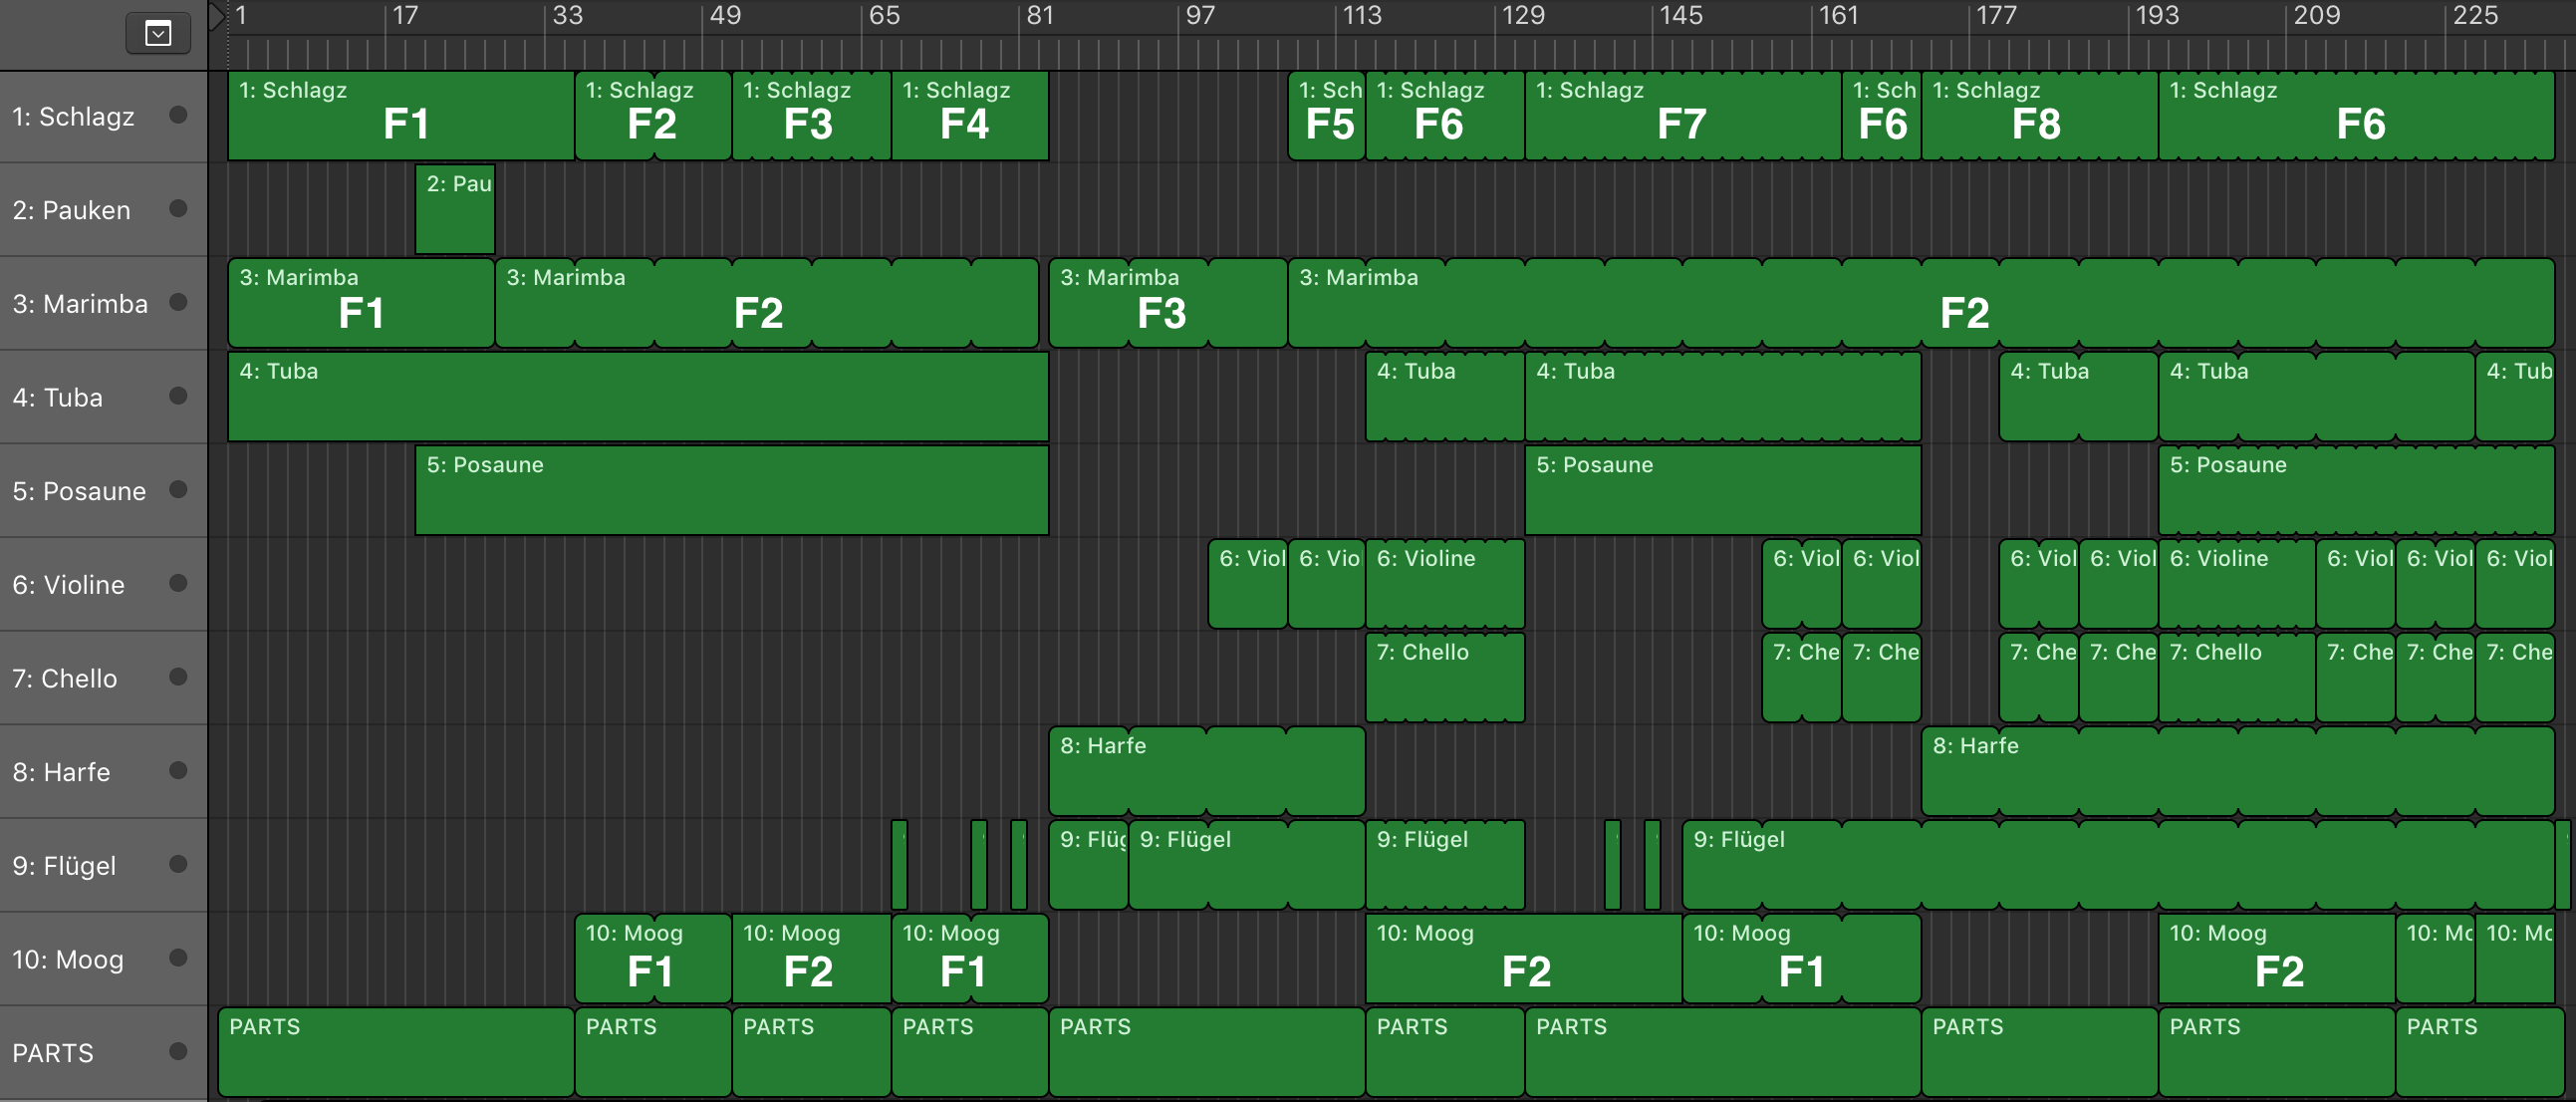
\includegraphics[width=0.99\columnwidth]{GlobaleStrukturMarkiert} 
	\caption{Globale Struktur dargestellt als leere MIDI-Regionen in Logic Pro mit Beschriftung der Figuren}
\end{figure}

\noindent Es wurde ebenfalls versucht die Abfolge mithilfe eines freien Notations-Programmes in einer Partitur darzustellen. Jedoch erwies sich die obige Darstellung als kompakter und ausreichend.

\section{Analyse und Synthese der einzelnen Instrumente}\
\textit{Abschnitt bearbeitet von: Raphael Drechsler}\\

\noindent Im folgenden Abschnitt sollen die zehn Instrumente synthetisiert werden. Wie in der globalen Struktur (siehe Abb. 1) zu erkennen ist, existieren in den meisten Fällen pro Instrument mehrere Figuren. Die folgenden Arbeitsschritte sollen daher pro Instrument und Figur erfolgen.

\paragraph{Analyse der gespielten Tonhöhen und Rhythmen.}  Diese Analyse erfolgt per Gehör. Untersucht wird dabei die Live-Version\cite{YT1} des Stückes. Für Parts, die besonders schwierig herauszuhören sind, da z.B. das Instrument nur sehr schwer hörbar ist, werden zusätzlich eine ähnliche Studio-Version\cite{YT2} sowie eine früher Variante\cite{YT3} des Liedes für die Untersuchung herangezogen.	Das Ergebnis der Analyse soll hier als Text, welcher die Figur beschreibt und/oder mithilfe von Noten dargestellt werden. 

\paragraph{Synthese von Tonhöhe und Rhythmus} Die analysierten Tonhöhen und Rhythmen sollen als Tidal Code umgesetzt werden. Dabei wird kein gesteigerter Wert auf die Auswahl eines passenden Klanges gelegt. Im Vordergrund der Betrachtung steht, dass der umgesetzte Code den analysierten Tonhöhen und Rhythmen entspricht. Vereinzelt soll hierbei auf zu überwindende Herausforderungen und genutzte Funktionen eingegangen werden.

\paragraph{Klanganalyse} Per Gehör soll das Klangbild des Instrumentes in der speziellen Figur sowie die Wirkung, die durch die Figur beim Hörer erzeugt wird untersucht werden. 

\paragraph{Anpassung der Klangsynthese} Unter Berücksichtigung des Analysierten Klangbildes und des bereits vorliegenden Tidal-Codes soll nun die Art der Klangsynthese derart angepasst werden, dass die Beschriebene klangliche Wirkung erzielt wird. Mögliche Arten der Anpassung sind dabei die Auswahl von Tidal-Instrumenten, Einbinden von Samples sowie Erstellen eines SuperCollider-Instrumentes.\\

\noindent Auf diesem Wege sollen die Figuren aller Instrumente als ausführbarer Tidal-Code mit erwünschter klanglicher Wirkung entstehen.
Das Verbinden der einzelnen Figuren zu einem live vorführbaren Stück soll in \textit{Kapitel 5 - Performance} beschrieben werden. 


%
%\subsection{Instrument 0: Was ist pro Instrument TODO?}
%{\color{red}\textbf{TODO}}: Nach Bearbeitung Hilfskapitel entfernen.\\
%
%Raph.\\
%Welche Figuren?
%- Welche Wirkung?
%- Welche Noten?\\
%
%Nico\\
%Wie klingt das Instrument?\\
%- Wie klingt das live? Einzelne Bestandteile? (Marimba gespielt mit Holzsticks und verschiedene Kuhglocken)
%- Wie klingt das in welcher Figur? (zB. BD laut, leise)
%- Welchen Klang wählen (evaluation - SD-Instrument nutzbar?, WAV suchen/selber aufnehmen, Instrument coden)\\

\subsection{Instrument 1: Schlagzeug}
\subsubsection{Figuren}
\textit{Abschnitt bearbeitet von: Raphael Drechsler}\\

\noindent \textbf{Figur 1}\\
Herausgehört wurde das folgende Muster. Die Note \textit{A} steht dabei für die Base-Drum, Note \textit{Dis} für die High-Hat.
\begin{figure}[h]
	\centering 
	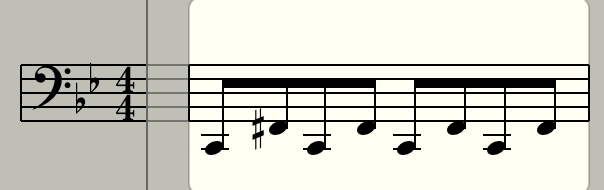
\includegraphics[width=0.3\columnwidth]{Drum_Fig1} 
	\caption{Schlagzeug Figur 1}
\end{figure}

\noindent Um in Tidal pro Takt eine Figur mit 4 Schlägen auf die Base-Drum und 4 Schlägen auf die High-Hat im Wechsel zu realisieren, lässt sich eine Kombination von Gruppierung und Wiederholung\cite{tid1} verenden:
\begin{lstlisting}
d1 $ sound "[bd hh]*4"
\end{lstlisting}

\noindent \textbf{Figur 2}\\
Herausgehört wurde eine Figur über 8 Takte. Dabei werden in Takt 3,7 und 8 wie nachfolgend notiert Fills auf der High-Hat gespielt.\\
\begin{figure}[h]
	\centering 
	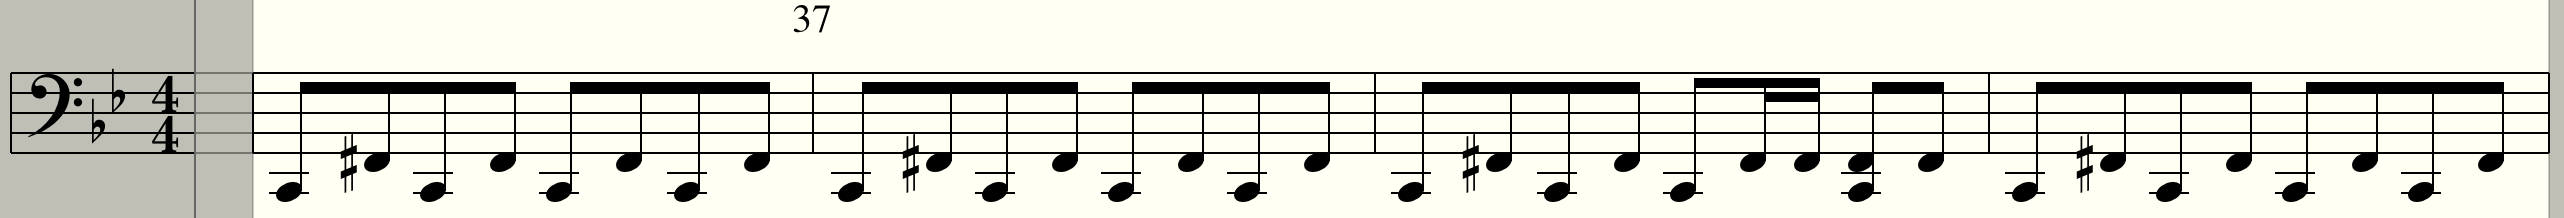
\includegraphics[width=0.8\columnwidth]{Drums_Fig2A} 
	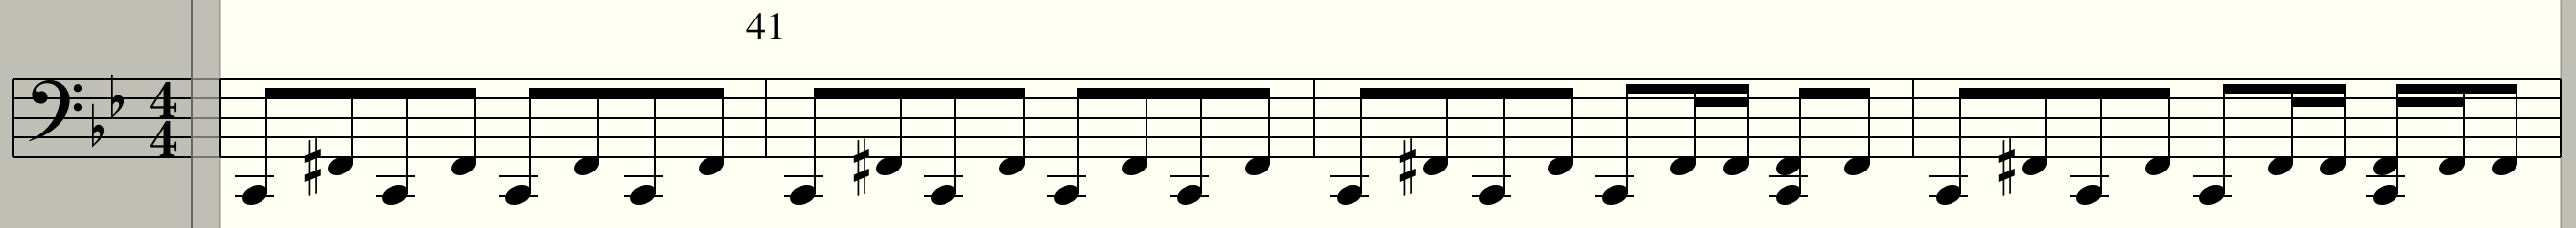
\includegraphics[width=0.8\columnwidth]{Drums_Fig2B} 
	\caption{Schlagzeug Figur 2}
\end{figure}

\noindent Die Umsetzung in Tidal der einzelnen Takte ohne Fills erfolgt analog zu Figur 1. In den Takten mit Fills werden auf einige Zählzeiten Base-Drum und High-Hat gleichzeitig gespielt. Dies kann in Tidal durch die Nutzung von   \verb1stack1 \cite{tid2} umgesetzt werden. Über den \verb1cat1-Ausdruck\cite{tid3} werden die acht Figuren hintereinander gespielt, was den Cycle auf die gewünschte Länge von acht Takten verlängert. Es ergibt sich folgender Code.

\begin{lstlisting}
d1 $  cat [
sound "[[bd hh]*4]",
sound "[[bd hh]*4]",
stack [ sound "[bd ~]*4", sound "[~ hh ~ hh][~ [hh hh] hh hh]" ],
sound "[[bd hh]*4]",
sound "[[bd hh]*4]",
sound "[[bd hh]*4]",
stack [ sound "[bd ~]*4", sound "[~ hh ~ hh][~ [hh hh] hh hh]" ],
stack [ sound "[bd ~]*4", sound "[~ hh ~ hh][~ [hh hh] [hh hh] hh]" ]
]
\end{lstlisting}

\noindent \textbf{Figur 3}\\
Herausgehört wurde die folgende Figur mit zwei Takten Länge. Die Note \textit{Fes} steht dabei für eine geöffnete High-Hat.
\begin{figure}[h]
	\centering 
	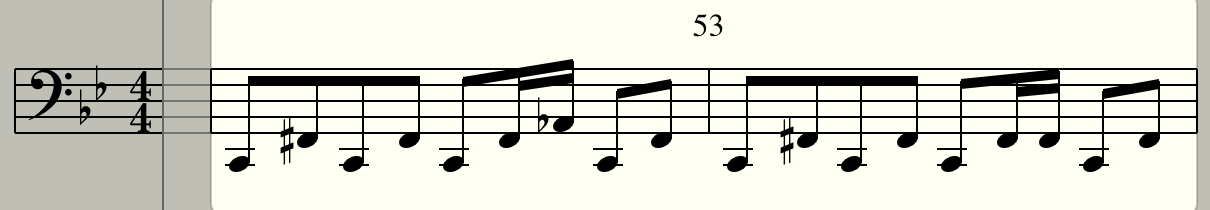
\includegraphics[width=0.5\columnwidth]{Drums_Fig3} 
	\caption{Schlagzeug Figur 1}
\end{figure}

\noindent In Tidal wurde die Figur hintereinander in Gruppierungen geschrieben und per \verb1slow 21\cite{tid4} auf die Länge von zwei Takten gestreckt.
\begin{lstlisting}
d1 $  slow 2 $ sound "[bd hh bd hh][bd [hh ho] bd hh] [bd hh bd hh][bd [hh hh] bd hh]"
\end{lstlisting}

\noindent \textbf{Figur 4}\\
Analog zu Figur 1. Dazu kommen zyklische Bewegung auf der Rim (Rand der Snare-Drum).
Die Figur ließ sich nur schwer durch Raushören bestimmen. Es wurden daher 5 Schläge auf die Rim pro Takt als Annahme getroffen, wobei aller 2 Takte der letzte Schlag ausgelassen wird.\\

\noindent Dies realisiert der folgende Tidal-Code.
\begin{lstlisting}
d1 $ stack [
sound "[bd hh]*4",
cat[sound "[rm rm rm rm rm]", sound "[rm rm rm rm ~]"] 
]
\end{lstlisting}

\noindent \textbf{Figur 5}\\
Nur die zyklische Rimclick-Bewegung aus Figur 4.
\begin{lstlisting}
d1 $ cat[sound "[rm rm rm rm rm]", sound "[rm rm rm rm ~]"]
\end{lstlisting}

\noindent \textbf{Figur 6 und 7}\\
Figur 6 wie Figur 4 und Figur 7 wie Figur 3. Jeweils kräftiger gespielt. Dies wird später in der Performance mit einem \verb1# gain1-Ausdruck\cite{tid5} zum Regulieren der Lautstärke des gespielten Samples umgesetzt.\\

\noindent \textbf{Figur 8}\\
Wie Figur 4 aber ohne Base-Drum.
\begin{lstlisting}
d1 $ stack [
sound "[~ hh]*4" ,
cat[sound "[rm rm rm rm rm]", sound "[rm rm rm rm ~]"] 
]
\end{lstlisting}

\subsubsection{Klangbild}
\textit{Abschnitt bearbeitet von: Nico Mehlhose}\\

\noindent Bestandteile des Schlagzeuges: herkömmliches Schlagzeug\\
Art der Synthetisierung: Da Bass Drum und High Head normal gespielt werden können die Sounds aus dem Supercollider 
mit minimaler Anpassung benutzt werden. Lediglich die Rim aus Figur 4 muss, wegen ihres hölzernen Sounds, selbst 
aufgenommen werden.\\
\noindent \textbf{Figur 1}\\
Sound BD: Base Drum wird mit zunehmender dauer lauter gespielt\\
Sound HH: wird Anfangs nur sanft angespielt aber mit zunehmender Zeit etwas lauter\\
Problem: Base Drum und High Hat müssen mit zunehmender Vorführungszeit lauter werden\\ 
Lösung: Die Lautstärkensteigerung der Schlagzeugs wird live mittels der Erhöhung des \textit{gain}-Parameters realisiert.\\
\begin{lstlisting}
Code: p "i1" $ sound "[bd hh]*4" #gain 0.9 # midinote 58
\end{lstlisting}
\noindent \textbf{Figur 2}\\
Sound: Das Schlagzeug wird in dieser Figur bis auf die Lautstärkensteigerung analog zu Figur 1 gespielt. In dieser Figur ist die Lautstärke gleichbleibend
und erhöht sich nicht.\\
Lösung:\\
\begin{lstlisting}
Code:\\
p "i1" $ cat [
sound "[[bd hh]*4]",
sound "[[bd hh]*4]",
stack [ sound "[bd ~]*4", sound "[~ hh ~ hh][~ [hh hh] hh hh]" ],
sound "[[bd hh]*4]",
sound "[[bd hh]*4]",
sound "[[bd hh]*4]",
stack [ sound "[bd ~]*4", sound "[~ hh ~ hh][~ [hh hh] hh hh]" ],
stack [ sound "[bd ~]*4", sound "[~ hh ~ hh][~ [hh hh] [hh hh] hh]" ]
] #midinote 58
\end{lstlisting}
\noindent \textbf{Figur 3}\\

{\color{red}\textbf{TODO}} Klangbild 3-8

Fig4:\\
Sound Rim: \\
Nico: selber bauen da keine hölzernen klänge vorhanden sind

Fig6:\\
irgendwas mit gain?\\



Töne: hh, bd (dumpf, wenig knackig)\\
rim

\subsection{Instrument 2: Pauken}
\subsubsection{Figuren}
{\color{red}\textbf{OFFEN}} \\
{\color{red}\textbf{TODO}}
(Hierzu Studio-Version hören)\\

\subsubsection{Klangbild}
Bestandteile der Pauke: 3 Kesselpauken\\
Art der Synthetisierung:?\\


\subsection{Instrument 3: Marimba}
\subsubsection{Figuren}
\textit{Abschnitt bearbeitet von: Raphael Drechsler}\\

\noindent \textbf{Figur 1}\\
Die Tonhöhe war per Gehör nicht genau differenzierbar. Es wurde folgende Annahme getroffen.
\begin{figure}[h]
	\centering 
	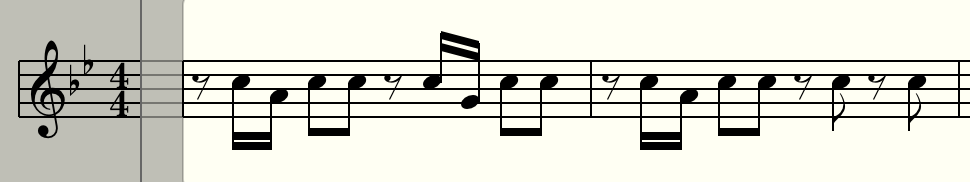
\includegraphics[width=0.5\columnwidth]{Marimba_Fig1} 
	\caption{Marimba Figur 1}
\end{figure}

\noindent Die Tonhöhe des Sounds \verb|glasstrap| wurde mithilfe des \verb|midinote|-Ausdrucks \cite{tid6} auf die jeweils gewünschte Tonhöhe geändert.
\begin{lstlisting}
p1 $ slow 2 $ midinote "[~ [51 49] 51 51][~ [51 46] 51 51][~ [51 49] 51 51][~ 51 ~ 51]" # s "glasstap"
\end{lstlisting}


\noindent \textbf{Figur 2}\\
In der Live-Version des Liedes ist im Video zu erkennen, dass auf der Marimba Kuhglocken (8 oder 10 Stück) in verschiedenen Tonhöhen liegen. Diese werden in der zweiten Figur auf die in der folgenden Abbildung gezeigten Zählzeit angespielt. Dabei wird Immer eine andere Tonhöhe gespielt. Das Muster in welcher Reihenfolge die Glocken gespielt werden wurde nicht weiter analysiert. Stattdessen soll das Anspielen der Glocken zur Vereinfachung randomisiert werden.
\begin{figure}[h]
	\centering 
	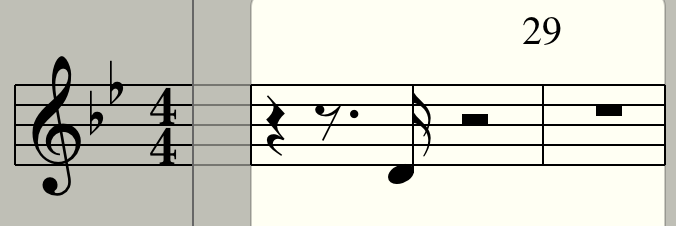
\includegraphics[width=0.25\columnwidth]{Marimba_Fig2} 
	\caption{Marimba Figur 2}
\end{figure}

\noindent Der Ausdruck \verb|irand 10| \cite{tid7} liefert einen zufälligen int-Wert von 0 bis einschließlich 9 zurück. Dieser Wert verändert in Verbindung mit dem \verb|# speed|-Ausdruck\cite{tid8} die Abspielgeschwindigkeit des \verb|can|-Samples und damit dessen Tonhöhe. So werden 9 verschiedene Kuhglocken simuliert.
\begin{lstlisting}
p1 $ stack [
slow 2 $ midinote "[~ [51 49] 51 51][~ [51 46] 51 51][~ [51 49] 51 51][~ 51 ~ 51]" # s "glasstap",
slow 2 $ midinote "[~[~~~60]~~][]" # s "can" # speed (1 + (irand 10)*0.2)
]
\end{lstlisting}

\noindent \textbf{Figur 3}\\
Es wurde folgende Figur per Gehör ermittelt. Dabei sind die Tonhöhen wie in Figur 1 angenommen.
\begin{figure}[h]
	\centering 
	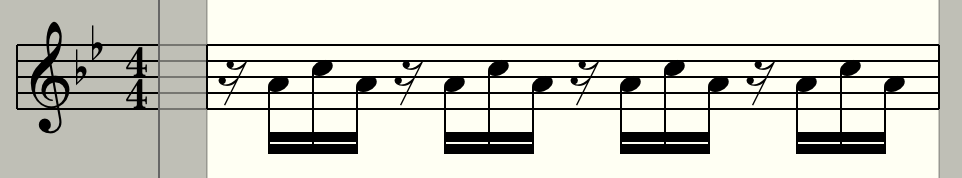
\includegraphics[width=0.5\columnwidth]{Marimba_Fig3} 
	\caption{Marimba Figur 3}
\end{figure}

\noindent Umsetzung in Tidal:
\begin{lstlisting}
p1 $ midinote "[~ 49 51 49]*4" # s "glasstap"
\end{lstlisting}


\subsubsection{Klangbild}
Bestandteile der Marimba: Eine Marimba, wobei Kuhglocken zum zufälligem Anspielen enthalten sind.\\
Art der Synthetisierung: Da keine hölzernen Klänge im SuperCollider enthalten sind müssen diese selbst aufgenommen werden. Dies geschieht mittels 
einem von \textit{SuperCollider Code} stammenden Code.{\color{red}\textbf{TODO}} Link einfügen\\
Für die Synthetisierung der Marimba mussten einige kleine Teilschritte unternommen werden. Zuerst die Syntetisierung des Moogs im SuperCollider.\\
Dazu wurde folgender Code von \textit{SuperCollider Code}{\color{red}\textbf{TODO}} Link einfügen kopiert und leicht abgewandelt, sodass er mer unseren Anforderungen entspricht:
\begin{lstlisting}
(
SynthDef(\bell, {
	|fs=1, t60=1, pitchy=1, amp=0.25, gate=1|
	var sig, exciter;
	//exciter = Impulse.ar(0);
	exciter = WhiteNoise.ar() * EnvGen.ar(Env.perc(0.001, 0.05), gate) * 0.25;
	sig = Klank.ar(
		`[
			[1, 2, 2.803, 3.871, 5.074, 7.81, 10.948, 14.421],   // freqs
			[1, 0.044, 0.891, 0.0891, 0.794, 0.1, 0.281, 0.079], // amplitudes
			[1, 0.205, 1, 0.196, 0.339, 0.047, 0.058, 0.047]*t60     // ring times
		],
		exciter,
		freqscale:fs*pitchy);
	sig = FreeVerb.ar(sig) * amp;
	DetectSilence.ar(sig, 0.001, 0.5, doneAction:2);
	Out.ar(0, sig!2);
}).add
)


(
Pbind(
	\instrument, \bell,
	\fs, 60.midicps,
	\t60, 0.45,
	\pitchy, 1.75,
	\dur, 0.25
).play;)

(
Pbind(
	\instrument, \bell,
	\fs, Pseq( (60..72), 1).midicps,
	\t60, 3,
	\pitchy, 2,
	\dur, 1
).play;
)

\end{lstlisting}
Wobei der erste Teil des Codes einen Ton erzeugt welcher Vergleichbar ist mit dem Kratzen auf einem Microphone.\\
Der zweite Teil ändert den ersten Sound so ab, sodass dieser mehr Hölzern klingt und der dritte Teil ist für den Sound der Glocken aus Figur 2.\\
Als nächstes muss dieser Sound aus dem SuperCollider aufgenommen werden. Dies geht mit dem Befehl \textit{Server.default.record;}.\\
Der dritte Schritt war das zuschneiden der Audisamples. Dazu wurde Audacity{\color{red}\textbf{TODO}} Link einfügen benutzt. Audacity ist ein kostenlosen Audioschnitt-, Editierungs- und Aufnahmeprogramm. Im Anschluss kann dann der Code für die einzelnen Figuren angepasst werden.\\
\noindent \textbf{Figur 1}\\
Sound Marimba: Die Marimba wird am Anfang des Stücks relativ dominant, im gegensatz zu den restlichen Instrumenten, gespiel\\
Lösung:\\
\begin{lstlisting}
p "i3" $ slow 2 $ midinote "[~ [59 57] 59 59][~ [59 54] 59 59][~ [59 57] 59 59][~ 59 ~ 59]" # s "Marimba" # room 0.5
\end{lstlisting}
\noindent \textbf{Figur 2}\\
Sound: Wird nur schwach angespielt wodurch sie in diesem Teil in den Hintergrund tritt.
Holzsticks auf Marimba in verschiedenen Tonhöhen wobei eher rhythmisch als melodisch eingesetzt, dazu Kuh-Glocken bereitstellen für Random-Funktion.\\
Lösung:\\
\begin{lstlisting}
p "i3" $ stack [
  slow 2 $ midinote "[~ [59 57] 59 59][~ [59 54] 59 59][~ [59 57] 59 59][~ 59 ~ 59]" # s "Marimba" # room 0.5,
  slow 2 $ sound "[ ~ [ ~ ~ ~ Glocken ] ~ ~ ][]" # n (irand 11) # cut 1
]
\end{lstlisting}
\noindent \textbf{Figur 3}\\
Sound: In der dritten Figur ist die Marimba nur sehr dezent im Hintergrund zu hören. Sie dient in dieser Figur lediglich als Taktgeber.\\
Lösung:\\
\begin{lstlisting}
p "i3" $ midinote "[~ 57 59 57]*4" # s "Marimba"
\end{lstlisting}
\subsection{Instrument 4: Tuba}
\subsubsection{Figuren}
\textit{Abschnitt bearbeitet von: Raphael Drechsler}\\

\noindent\textbf{Figur 1}\\
Es wurde eine Figur über einen Takt ermittelt, in der ein Schlag auf das Mundstück der Tube als rhythmisches Element auf zweite Zählzeit im Takt erfolgt.\\
\begin{figure}[h]
	\centering 
	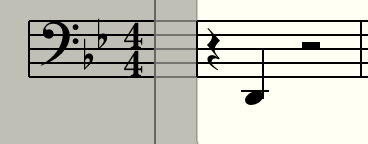
\includegraphics[width=0.25\columnwidth]{Tuba_Fig1} 
	\caption{Tuba Figur 1}
\end{figure}

\begin{lstlisting}
d1 $ sound "[~ sn ~ ~]"
\end{lstlisting}

\subsubsection{Figuren}
\textbf{Figur 2}\\
Es wurde eine Figur über 2 Takte ermittelt. Instrumentalist bläst in dieser Figur in die Tuba ohne dass die Lippen vibrieren, um ein Rauschen zu erzeugen. Am Ende der Figur wurde eine Pause als Atempause angenommen. 

\begin{figure}[h]
	\centering 
	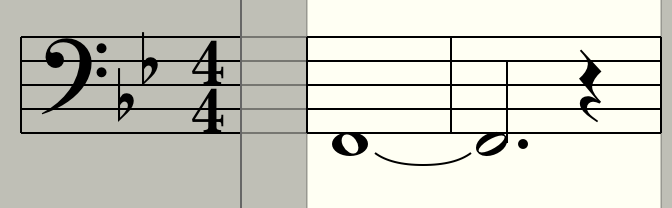
\includegraphics[width=0.25\columnwidth]{Tuba_Fig2} 
	\caption{Tuba Figur 2}
\end{figure}

\noindent Für die Umsetzung wird ein Sample benötigt, welches über die Dauer von zwei Takten reicht. Um dieses nur aller 2 Takte abzuspielen damit sich mehre Instanzen des Samples nicht überlagern kann der Ausdruck \verb|loopAt 2| \cite{tid9} verwendet werden.
\begin{lstlisting}
d1 $ loopAt 2 $ sound "blasesoundTuba"
\end{lstlisting}

\noindent\textbf{Figur 3}\\
Analyse-Ergebnis: Wie Figur 1, hier allerdings kurzes tonloses Pusten stoßweise gespielt anstelle von Schlag auf Mundstück. Code analog zu Figur 1.\\

\noindent\textbf{Figur 4}\\
Analyse-Ergebnis: Tiefe Töne durch Tuba. Die Tonhöhe ist nahezu nicht erkennbar. Die Tonhöhe wurde jedoch durch die Analyse in Figur 6 ableitbar. Die gespielten Töne werden über den Verlauf von zwei Durchläufen der Figur langsam lauter.\\

\begin{figure}[h]
	\centering 
	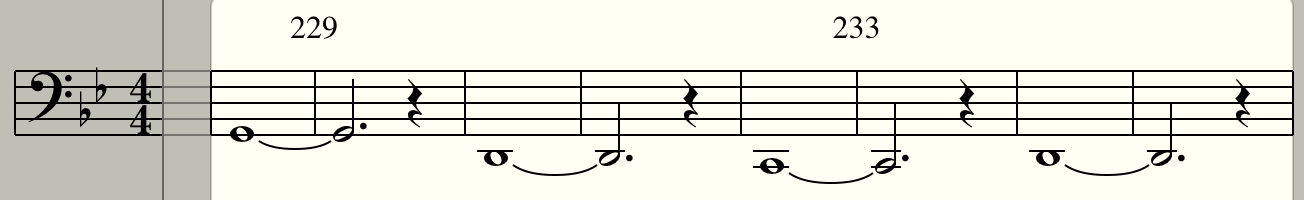
\includegraphics[width=0.7\columnwidth]{Tuba_Fig4} 
	\caption{Tuba Figur 4}
\end{figure}

\noindent Das lauter Werden der Töne über die Dauer von zwei Durchläufe der Figur wurde mit einem Pattern realisiert, welches dem \verb|# gain|-Effekt übergeben wurde.\cite{tid10} Um die lang ausgehaltenen Noten umzusetzen, wurde auf den Ausdruck ein Hall angewendet, wobei \verb|# room| die Lautstärke des Halls und \verb|# sz| die Größe des hallenden Raumes bedingt. \verb|# orbit 1| wird genutzt, um die ansonsten globale Wirkung des Hall-Effektes auf den vorangegangenen Ausdruck zu beschränken. \cite{tid11} 

\begin{lstlisting}
d1 $ slow 16 $ midinote "[43 38 36 38]*2" # s "superpiano" # room 0.85 # sz 0.8 # orbit 1 #gain "0.4 0.45 0.5 0.55 0.6 0.7 0.8 0.9"
\end{lstlisting}


\noindent\textbf{Figur 5}\\
Herausgehört wurde eine Figur analog zu Figur 4, jedoch kräftig gespielt.\\

\noindent\textbf{Figur 6}\\
Herausgehört wurde eine Figur analog zu Figur 5, jedoch maximal kraftvoll ausgespielt. Dabei werden die Töne jeweils eine Oktave höher gespielt, was die Tonhöhe der einzelnen Töne gut erkennbar macht.\\

\noindent Umsetzung in Tidal:
\begin{lstlisting}
d1 $ slow 8 $ midinote "55 50 48 50" # s "superpiano" # room 0.85 # sz 0.8 # orbit 1
\end{lstlisting}

\subsubsection{Klangbild}
\textit{Abschnitt bearbeitet von: Nico Mehlhose}\\
\noindent Bestandteile der Tuba: normale Tuba, welche aber entartet benutzt wird\\
Art der Synthetisierung: Da die Tuba ein reales Musikinstrument ist, welches in dieser Form nicht im Supercollider enthalten ist,
werden hierfür Samples benutzt. Die Samples werden für die entartete Benutzung in Tidal so manipuliert, dass sie die Sounds
nachempfinden.\\
Für Figur 2 wurde mit weit gespreitzten Nasenflügeln ausgeatmet und für Figur 3 wurde ein Handscheibenwischer mit hohlem Griff angespielt.\\

\noindent\textbf{Figur 1}\\
 Sound: In dieser Figur wird auf das Mundstück der Tuba geschlagen. Der erzeugte Ton hört sich in etwa an wie eine Base Drum ohne Bass.\\
Lösung:\\
\begin{lstlisting}
d1 $ sound "~ bd ~ ~" # midinote 15
\end{lstlisting}

\noindent\textbf{Figur 2}\\
Sound: ähnlich eines Reifens der Luft verliert\\
Lösung:Der Hall sorgt dafür, dass sich der Sound nach einem größerem Gegenstand und nicht nach einer Nase anhört.\\
\begin{lstlisting}
p "i4" $ loopAt 2 $ sound "Atmen" # room 1
\end{lstlisting}

\noindent\textbf{Figur 3}\\
Sound: Wie Sound aus Figur 2 aber mit mehr Druck und nicht durchgehend.\\
Lösung: \textit{Room} und \textit{Gain} haben hier den selben Effekt wie in Figur 2\\
\begin{lstlisting}
p "i4" $ sound "[~ Tuba ~ ~]" # room 0.4 # gain 1.1
\end{lstlisting}
\noindent\textbf{Figur 4, 5, 6}\\
Sound: Die Tuba wird in Figur 4 mit absteigender Lautstärke gespielt. In Figur 5 und 6 wird sie mit gleichbleibender Lautstärke gespielt wobei jedoch die Lautstärke
zwischen den Figuren ansteigt.\\
Lösung Figur 4:\\
\begin{lstlisting}
p "i4" $ slow 16 $ sound "[TubaOrch:20 TubaOrch:20 TubaOrch:20 TubaOrch:20]*2" # cut 1 #gain " 0.8 0.75 0.7 0.65 0.6 0.5 0.5 0.5"
\end{lstlisting}
Lösung Figur 5:\\
\begin{lstlisting}
p "i4" $ slow 16 $ sound "[TubaOrch:20 TubaOrch:20 TubaOrch:20 TubaOrch:20]*2" # cut 1 
\end{lstlisting}
Lösung Figur 6:\\
\begin{lstlisting}
p "i4" $ slow 16 $ sound "[TubaOrch:20 TubaOrch:20 TubaOrch:20 TubaOrch:20]*2" # cut 1 #gain 1.3
\end{lstlisting}

\subsection{Instrument 5: Posaune}
\subsubsection{Figuren}
\textit{Abschnitt bearbeitet von: Raphael Drechsler}\\

\noindent\textbf{Figur 1}\\
Herausgehört wurde eine Figur über einen Takt. In der Figur erfolgt ein kurzes, tonloses Pusten in die Posaune. Dieses wird Stoßweise gespielt und als rhythmisches Element auf letzte Achtelnote im Takt eingesetzt.\\
\begin{figure}[h]
	\centering 
	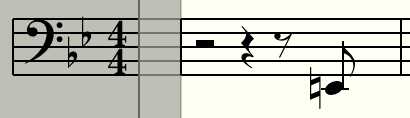
\includegraphics[width=0.25\columnwidth]{Posaune_Fig1} 
	\caption{Posaune Figur 1}
\end{figure}

\noindent Umsetzung in Tidal:
\begin{lstlisting}
d1 $ sound "[][[][~ sn]]"
\end{lstlisting}


\noindent\textbf{Figur 2}\\
Zu hören ist, dass die Figur ein Rauschen analog zur Figur 2 der Tuba umfasst. Der Code gestaltet sich entsprechend.
\begin{lstlisting}
d1 $ loopAt 2 $ sound "blasesoundPosaune"
\end{lstlisting}

\subsubsection{Klangbild}
Bestandteile der Posaune: normale Posaune, welche aber entartet benutzt wird.\\
Art der Synthetisierung: Da die Posaune ein reales Musikinstrument ist, welches in dieser Form nicht im Supercollider enthalten ist,
werden hierfür Samples benutzt. Die Samples werden eigens dafür aufgenommen. Die Sound werden wie bei der Tuba erzeugt.

\noindent\textbf{Figur 1}\\
 Sound: In dieser Figur wird auf das Mundstück der Posaune stoßartig angespielt.\\
Lösung:\\
\begin{lstlisting}
p "i5" $ sound "[][[][~ Posaune]]" # room 0.3 # gain 1.1
\end{lstlisting}

\noindent\textbf{Figur 2}\\
Sound: ähnlich zu Figur 3 der Tuba allerdings mit weniger tief.\\
Lösung: Für die geringere Tiefe des Sounds wurde der Hall der Posaune angepasst \\
\begin{lstlisting}
p "i5" $ loopAt 2 $ sound "Atmen" #room 0.7 # gain 1.1
\end{lstlisting}

\subsection{Instrument 6: Violine}
\subsubsection{Figuren}
\textit{Abschnitt bearbeitet von: Raphael Drechsler}\\

\noindent\textbf{Figur 1}\\
Herausgehört wurde die folgende Figur über 16 Takte.
\begin{figure}[h]
	\centering 
	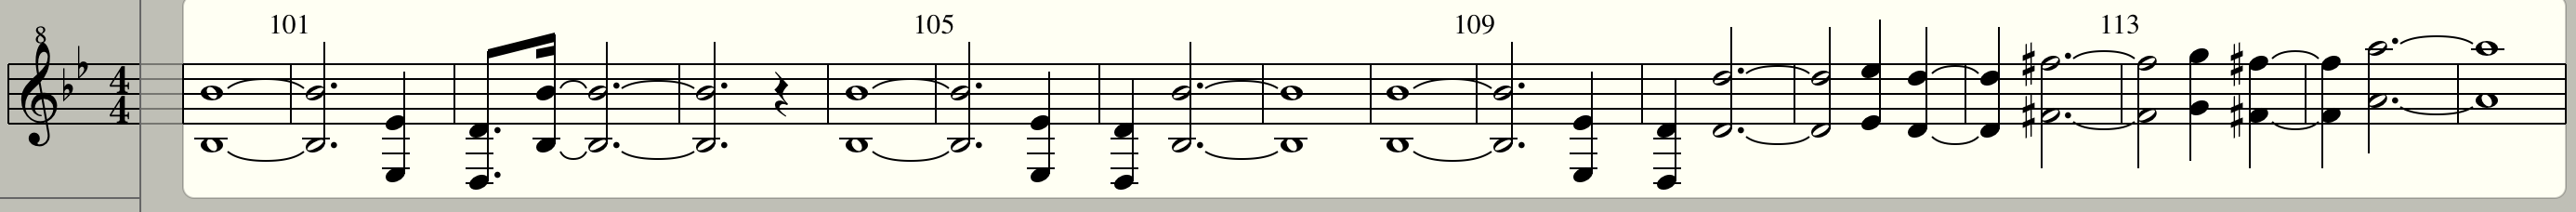
\includegraphics[width=0.99\columnwidth]{Violin_Fig1} 
	\caption{Violine Figur 1}
\end{figure}

\noindent Die Noten der Figur werden oktaviert gespielt. Der Einfachheit halber wurden nur die gut hörbaren hohen töne umgesetzt. Um jeweils einen Ton zu einem Zeitpunkt zu hören, werden die abgespielten Samples mithilfe des Ausdrucks \verb|# cut 1| immer dann gestoppt, sobald sie für den nächsten Ton abgespielt werden.\cite{tid12}

\begin{lstlisting}
d1 $ slow 4 $ cat [
midinote "[82][][][][][][][75][74][82][][][][][][]" # s "gtr",
midinote "[82][][][][][][][75][74][82][][][][][][]" # s "gtr",
midinote "[82][][][][][][][75][74][86][][][][][87][86]" # s "gtr",
midinote "[][90][][][][][91][90][][93][][][][][][]" # s "gtr"
] #cut 1 # room 0.85 # sz 0.8 # orbit 1 
\end{lstlisting}\

\noindent\textbf{Figur 2}\\
Analyse-Ergebnis:
\begin{figure}[h]
	\centering 
	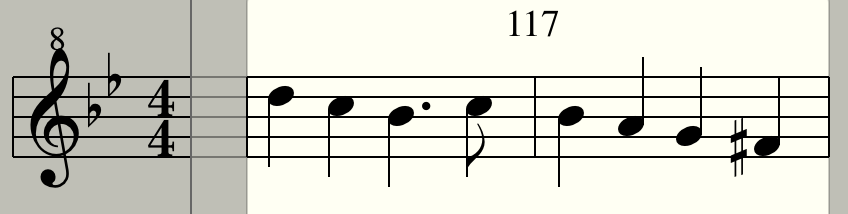
\includegraphics[width=0.3\columnwidth]{Violin_Fig2} 
	\caption{Violine Figur 2}
\end{figure}

\noindent Umsetzung in Tidal:
\begin{lstlisting}
$ slow 2 $ midinote "[[86][84][82][[][84]]][82 81 79 78]" # s "gtr" #cut 1 # room 0.85 # sz 0.8 # orbit 1
\end{lstlisting}

\noindent\textbf{Figur ?}\\
{\color{red}\textbf{TODO}} weitere Figuren im hinteren Teil des Stückes

\subsubsection{Klangbild}
{\color{red}\textbf{TODO}}auf Raphas Meinung warten
Bestandteile der Violine: Violine\\
Art der Synthetisierung: Hierfür wurden Samples Online gesucht da wir möglichs viele verschiedene Arten der Soundeinbindung abdecken wollten. Dabei wurde ein großer Datenbestand von Orchesterinstumenten gefunden.{\color{red}\textbf{TODO}}http://virtualplaying.com/virtual-playing-orchestra/ Link einfügen Des weiteren
wäre es extremst Zeitaufwendig jedes Instrument über den SuperCollider zu synthetisieren weshalb Sound Samples für dieses Instrument gewählt wurden.\\
\noindent\textbf{Figur 1}\\
Sound: In dieser Figur steigt die Violine leise in das Stück ein und wird über die Zeit immer lauter, wodurch sie schlussendlich im zweiten Teil 
zum Hauptinstrument des Abschnittes wird. Im ersten Teil wird die Violine etwas quitschend und langsam gespielt. Im zweiten Teil wird sie hektisch und sauber gespielt.\\
Problem: Die Violine muss in unserer Vorführung diesen gleichmäßigen Anstieg der Lautstärke vollführen, ohne merkliche Sprünge zu machen.\\
Lösung:\\
\begin{lstlisting}
p "i6" $ slow 16 $ fastcat [
midinote "[52][][][][][][][45][44][52][][][][][][]" # s "Violine:5",
midinote "[52][][][][][][][45][44][52][][][][][][]" # s "Violine:5",
midinote "[52][][][][][][][45][44][56][][][][][57][56]" # s "Violine:5",
midinote "[][60][][][][][61][60][][63][][][][][][]" # s "Violine:5"
]  #gain 0.5 #cut 1 #speed 1.2 # sz 0.8 # orbit 1 # room 0.85

\end{lstlisting}
\noindent\textbf{Figur 2}\\
Sound: Wenn die Violine in diese Figur übergeht ist sie das Hauptinstrument des Stückes. Die Violine wird hierbei sehr hektisch aber im gegensatz zu Figur 1 sauber gespielt.\\
Lösung:\\
\begin{lstlisting}
p "i6" $ slow 2 $ midinote "[[62][60][58][[][60]]][58 57 55 54]" # s "Violine:6" #cut 1 # room 0.85 # sz 0.8 # orbit 1 # speed 1.5
\end{lstlisting}



\subsection{Instrument 7: Chello}
\subsubsection{Figuren}
\textit{Abschnitt bearbeitet von: Raphael Drechsler}\\

\noindent\textbf{Figur 1}\\
Analyse-Ergebnis:
\begin{figure}[h]
	\centering 
	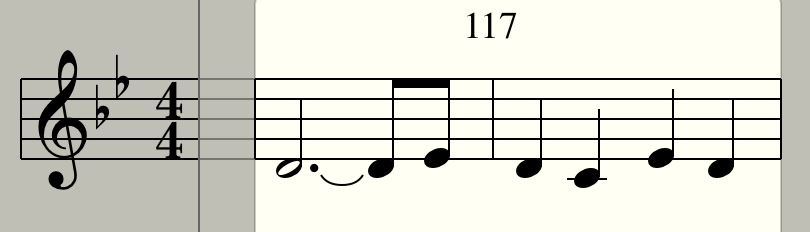
\includegraphics[width=0.3\columnwidth]{Chello_Fig1} 
	\caption{Chello Figur 1}
\end{figure}

\noindent Umsetzung in Tidal:
\begin{lstlisting}
p1 $ slow 2 $ midinote "[[74][][][[][75]]][74 72 75 74]" # s "gtr" #cut 1 # room 0.85 # sz 0.8 # orbit 1
\end{lstlisting}

\noindent\textbf{Figur 2}\\
Analyse-Ergebnis:
\begin{figure}[h]
	\centering 
	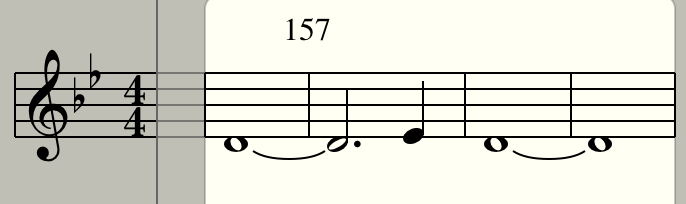
\includegraphics[width=0.3\columnwidth]{Chello_Fig2} 
	\caption{Chello Figur 2}
\end{figure}

\noindent Umsetzung in Tidal:
\begin{lstlisting}
p1 $ slow 4 $ midinote "[[62][[][][][63]]][62]" # s "gtr" #cut 1 # room 0.85 # sz 0.8 # orbit 1
\end{lstlisting}

\noindent\textbf{Figur ?}\\
{\color{red}\textbf{TODO}} weitere Figuren im hinteren Teil des Stückes

\subsubsection{Klangbild}
{\color{red}\textbf{TODO}}Figuren einarbeiten, WIE ZUM FICK SOLL ICH DA EIN CELLO RAUSHÖREN ICH HÖRE DA GARNICHTS *gnarf*\\
Bestandteile: Cello\\
Art der Synthetisierung: Das Cello wird wie auch die Violine über die Samples realisiert{\color{red}\textbf{TODO}} Quelle einfügen, welches anschließend in den SuperCollider eingefügt wird, synthetisiert.
Ruhige Parts, Hektik (schnell gespielte Töne)

\noindent\textbf{Figur 1}\\
Lösung:\\
\begin{lstlisting}
p "i7" $ slow 2 $ midinote "[[54][][][[][55]]][54 52 55 54]" # s "Cello:1" #cut 1 # room 0.85 # sz 0.8 # orbit 1 #gain 0.7
\end{lstlisting}
\noindent\textbf{Figur 2}\\
Lösung:\\
\begin{lstlisting}
p "i7" $ slow 4 $ midinote "[[42][[][][][43]]][42]" # s "Cello:2" #cut 1 # room 0.85 # sz 0.8 # orbit 1 #gain 0.7
\end{lstlisting}

\subsection{Instrument 8: Harfe}
\subsubsection{Figuren}
\textit{Abschnitt bearbeitet von: Raphael Drechsler}\\

\noindent\textbf{Figur 1}\\
Die Rhythmik sowie die Tonhöhe der zweitaktigen Figur ließen sich nicht ohne weiteres bestimmen. Zur Reduzierung des Arbeitsaufwandes wurde für die Figur die folgende Annahme getroffen. 
\begin{figure}[h]
	\centering 
	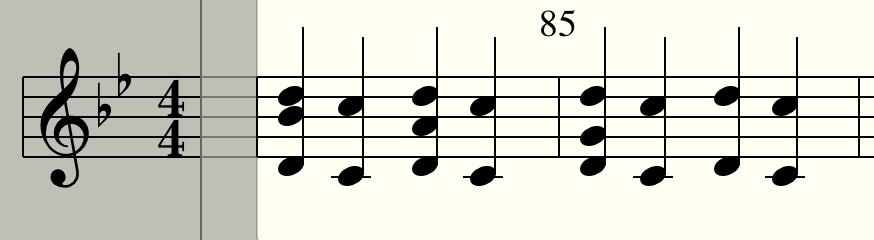
\includegraphics[width=0.3\columnwidth]{Harp_Fig1} 
	\caption{Harfe Figur 1}
\end{figure}

\noindent Umsetzung in Tidal:
\begin{lstlisting}
d1 $ stack [
  midinote "[74 72]*2" # s "gtr",
  midinote "[62 60]*2" # s "gtr",
  cat [
    midinote "70 69" # s "gtr",
    midinote "67" # s "gtr",
    midinote "70 69" # s "gtr",
    midinote "66" # s "gtr"
  ]
] 
\end{lstlisting}



\subsubsection{Klangbild}
{\color{red}\textbf{TODO}} Art der Synthetisierung anpassen
Bestandteile der Harfe: Harfe\\
Art der Synthetisierung: Die Harfe wird mit Samples synthetisiert da diese nicht über die SuperCollidertöne synthetisierbar ist.\\
Sound: Die Harfe wird in ihren Teilen sehr deutlich gespielt. Jedoch schwankt die Lautstärke mit der sie gespielt wird von leise zu laut und wieder zurück.\\
Problem: Die schwankende Lautstärke ist das Hauptproblem bei der Aufführung.\\
Lösung:\\
\begin{lstlisting}
\\
\end{lstlisting}


\subsection{Instrument 9: Flügel}
\subsubsection{Figuren}
\textit{Abschnitt bearbeitet von: Raphael Drechsler}\\

\noindent\textbf{Figur 1}\\
Analyse-Ergebnis:
\begin{figure}[h]
	\centering 
	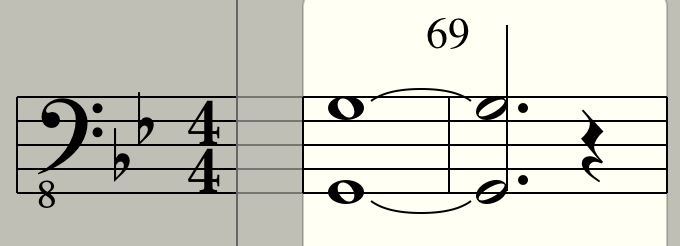
\includegraphics[width=0.3\columnwidth]{Flug_Fig1} 
	\caption{Flügel Figur 1}
\end{figure}
\noindent Umsetzung in Tidal:
\begin{lstlisting}
p1 $ slow 2 $ stack[midinote "43 " #s "superpiano", midinote "55 " #s "superpiano"]
\end{lstlisting}

\noindent \textbf{Figur 2}\\
Analyse-Ergebnis:
\begin{figure}[h]
	\centering 
	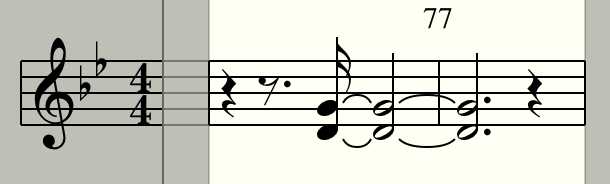
\includegraphics[width=0.3\columnwidth]{Flug_Fig2} 
	\caption{Flügel Figur 2}
\end{figure}\\
\noindent Umsetzung in Tidal:
\begin{lstlisting}
p1 $ slow 2 $ stack[
  midinote "[[][[][][][67]][][]][]" #s "superpiano",
  midinote "[[][[][][][62]][][]] []" #s "superpiano"
] # room 0.5 # sz 0.83 # orbit 1
\end{lstlisting}

\noindent \textbf{Figur 3}\\
Analyse-Ergebnis:
\begin{figure}[h]
	\centering 
	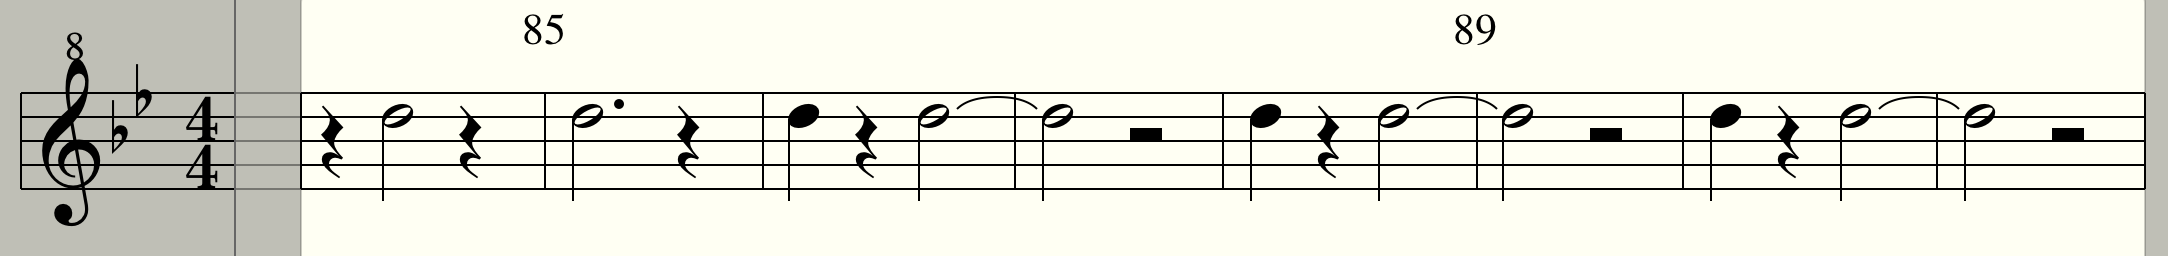
\includegraphics[width=0.8\columnwidth]{Flug_Fig3} 
	\caption{Flügel Figur 3}
\end{figure}

\noindent Umsetzung in Tidal:
\begin{lstlisting}
p1 $ slow 2 $ midinote "[86 ~][86][~] [~] " # s "superpiano"  # room 0.5 # sz 0.83 # orbit 1 #gain "<0.65 0.7 0.75 0.8>"
\end{lstlisting}


\noindent \textbf{Figur 4}\\
Analyse-Ergebnis:
\begin{figure}[h]
	\centering 
	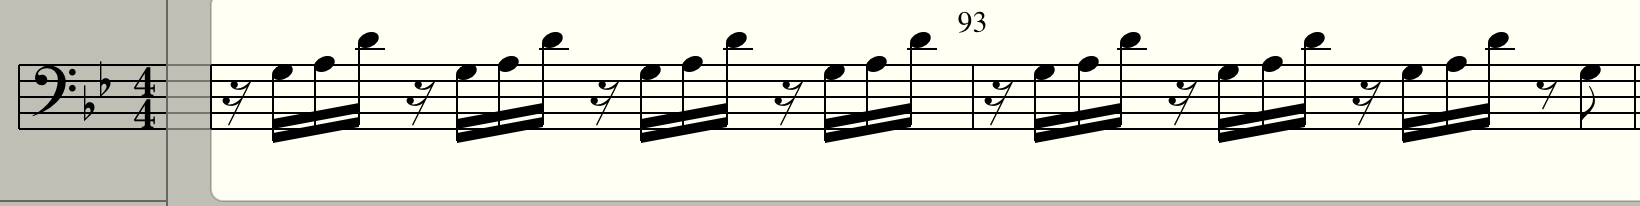
\includegraphics[width=0.9\columnwidth]{Flug_Fig4a} 
	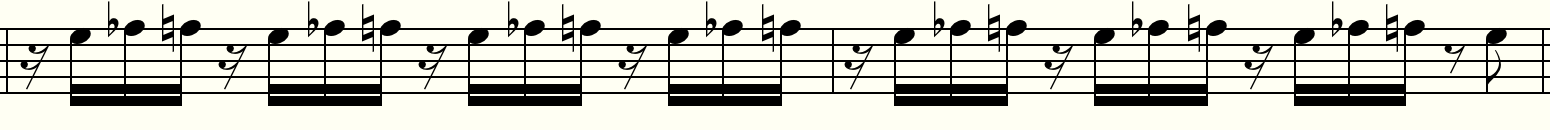
\includegraphics[width=0.9\columnwidth]{Flug_Fig4b} 
	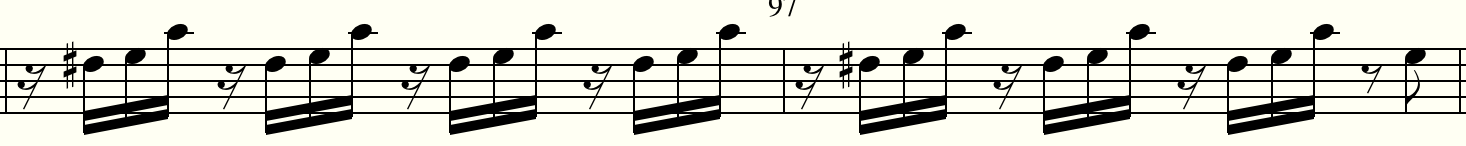
\includegraphics[width=0.9\columnwidth]{Flug_Fig4c} 
	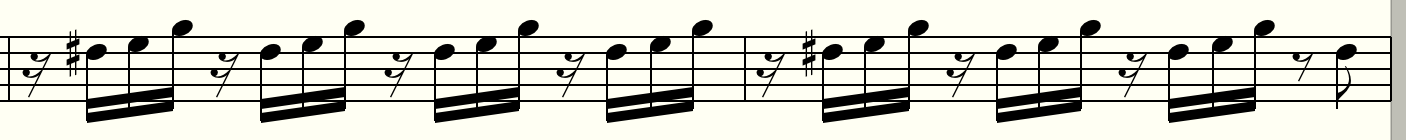
\includegraphics[width=0.9\columnwidth]{Flug_Fig4d} 
	\caption{Flügel Figur 4}
\end{figure}

\noindent Umsetzung in Tidal:
\begin{lstlisting}
d1 $ slow 2 $ cat [
midinote "~ 67 69 74 ~ 67 69 74 ~ 67 69 74 ~ 67 69 74 ~ 67 69 74 ~ 67 69 74 ~ 67 69 74  ~ ~ 67 ~ " # s "superpiano",
midinote "~ 67 68 69 ~ 67 68 69 ~ 67 68 69 ~ 67 68 69 ~ 67 68 69 ~ 67 68 69 ~ 67 68 69  ~ ~ 67 ~ " # s "superpiano",
midinote "~ 66 67 72 ~ 66 67 72 ~ 66 67 72 ~ 66 67 72 ~ 66 67 72 ~ 66 67 72 ~ 66 67 72  ~ ~ 67 ~ " # s "superpiano",
midinote "~ 66 67 70 ~ 66 67 70 ~ 66 67 70 ~ 66 67 70 ~ 66 67 70 ~ 66 67 70 ~ 66 67 70  ~ ~ 66 ~ " # s "superpiano"
]
\end{lstlisting}

\noindent \textbf{Figur 5}\\
Analyse-Ergebnis:
\begin{figure}[h]
	\centering 
	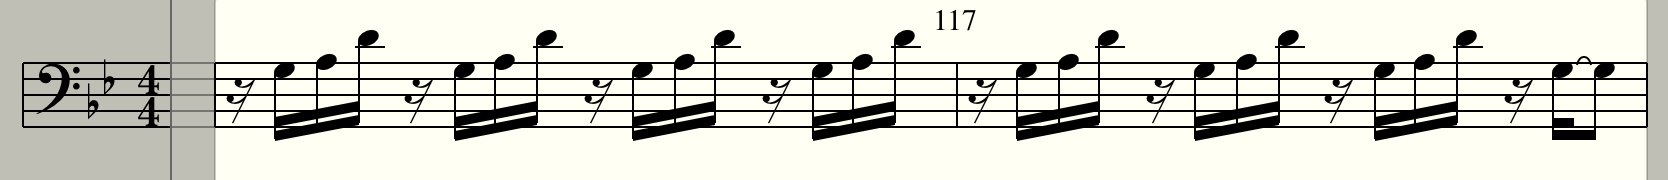
\includegraphics[width=0.9\columnwidth]{Flug_Fig5} 
	\caption{Flügel Figur 5}
\end{figure}

\noindent Umsetzung in Tidal:
\begin{lstlisting}
d1 $ slow 2 $ midinote "~ 67 69 74 ~ 67 69 74 ~ 67 69 74 ~ 67 69 74 ~ 67 69 74 ~ 67 69 74 ~ 67 69 74  ~ ~ 67 ~ " # s "superpiano"
\end{lstlisting}


\subsubsection{Klangbild}
{\color{red}\textbf{TODO}}vllt auch aufnehmen?
Bestandteile des Flügels: Flügel\\
Art der Synthetisierung:?\\
\noindent \textbf{Figur 1}\\
Sound: Der Sound der Figur wird zur Einleitung in den ersten Hauptabschnitt benutzt. Dabei werden die Tasten des Flügels 
schnell gedrückt um einen möglichst lauten Ton hervorzubringen.\\
Lösung:\\
\begin{lstlisting}
\\
\end{lstlisting}
\noindent \textbf{Figur 2}\\
Sound: Der Flügel wird in dieser Figur normal angespielt und führt den Zuhörer zu dem Höhepunkt des ersten Haupteiles welcher von der Violine gespielt wird.\\
Lösung:\\
\begin{lstlisting}
\\
\end{lstlisting}
\noindent \textbf{Figur 4}\\
Sound: normal angespielter Flügel\\
Lösung:\\
\begin{lstlisting}
\\
\end{lstlisting}

\subsection{Instrument 10: Moog Syntheziser}
\subsubsection{Figuren}
\textit{Abschnitt bearbeitet von: Raphael Drechsler}\\

\noindent\textbf{Figur 1}\\
Herausgehört wurde der folgende Basslauf über acht Takte.\\
\begin{figure}[h]
	\centering 
	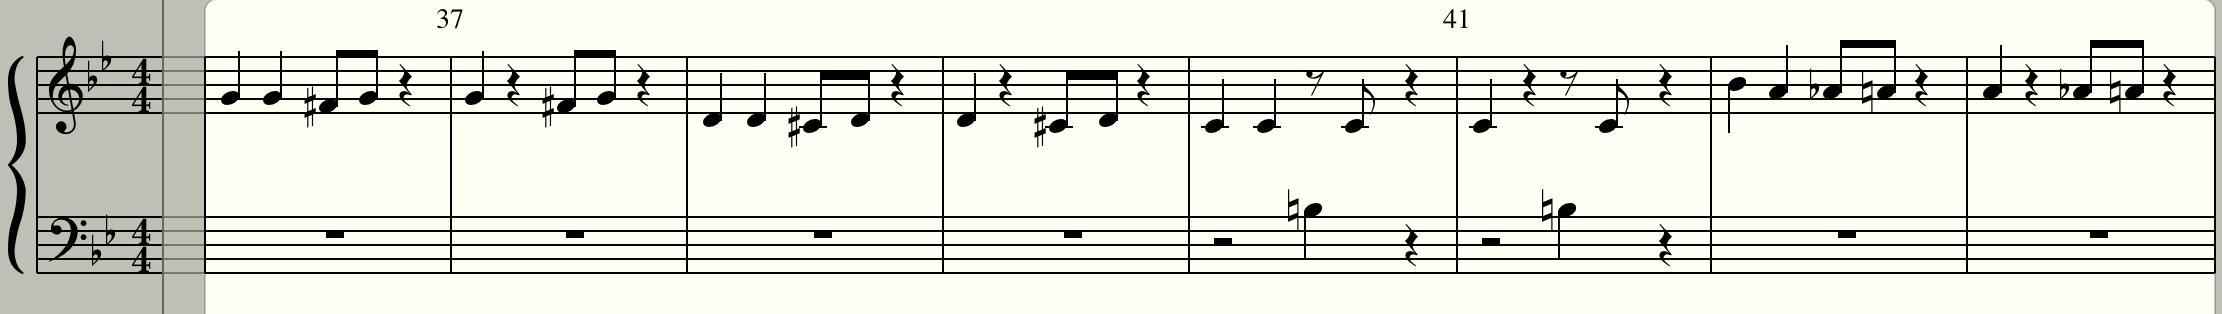
\includegraphics[width=1\columnwidth]{Bass_Fig1} 
	\caption{Moog Figur 1}
\end{figure}

\noindent Umsetzung in Tidal:
\begin{lstlisting}
d1 $ slow 2 $ cat [
  midinote "[[55 55][54 55 ~ ~]]*2" # s "moog",
  midinote "[[50 50][49 50 ~ ~]]*2" # s "moog",
  midinote "[[48 48][47 48 ~ ~]]*2" # s "moog",
  midinote "[[58 57][56 57 ~ ~]]  [[57 ~][56 57 ~ ~]]" # s "moog" 
] # cut 1
\end{lstlisting}

\noindent\textbf{Figur 2}\\
Herausgehört wurde der folgende Basslauf über einen Takt.
\begin{figure}[h]
	\centering 
	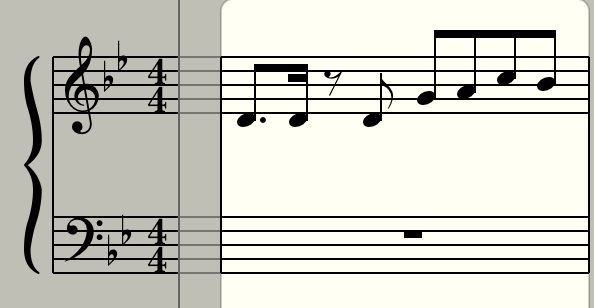
\includegraphics[width=0.3\columnwidth]{Bass_Fig2} 
	\caption{Moog Figur 2}
\end{figure}

\noindent Umsetzung in Tidal:
\begin{lstlisting}
d1 $ midinote "[[[[50 ~ ~ 50]][~ 50]][55 57 60 58]]" # s "moog" # cut 1
\end{lstlisting}

\subsubsection{Klangbild}
{\color{red}\textbf{TODO}} Nochmal umschreiben wegen Marimba
Bestandteile des Moogs: Keyboard, PC, Mischboard\\
Art der Synthetisierung: Der Moog wird von uns selbst im SuperCollider Programmiert, da ein Moog relativ leicht selbst zu Programmieren ist.
Des weiteren wollen wir uns damit die Option offen halten anstatt eines Moogs eine Bassline zu benutzen.\\ \\

Für die Synthetisierung des Moogs mussten einige kleine Teilschritte unternommen werden. Zuerst die Syntetisierung des Moogs im SuperCollider.\\
Dazu wurde folgender Code geschrieben:
\begin{lstlisting}
x=(
SynthDef(\moog, {
	arg freq=102, width=0.5, mul=0.5, freq2=300, q=0.2, mode=0;
	var moog ;
	
		moog=BMoog.ar(Pulse.ar(freq,width,  mul),freq2, q, mode, mul:0.2);
		
		
		Out.ar(0, moog);
		Out.ar(1, moog);
	
}).play
)
\end{lstlisting}
Als nächstes muss dieser Sound aus dem SuperCollider aufgenommen werden. Dies geht mit dem Befehl \textit{Server.default.record;}.\\
Der dritte und letzte Schritt war das zuschneiden der Audisamples. Dazu wurde Audacity benutzt. Danach kann dann der Code für die einzelnen Figuren angepasst werden.\\
\noindent\textbf{Figur 1}\\
Lösung:\\
\begin{lstlisting}
p "i10" $ slow 8 $ fastcat [sound "[[BBFMoog:5 BBFMoog:5][BBFMoog:4 BBFMoog:5 ~ ~]]*2" # cut 1 ,
sound "[[BBFMoog:3 BBFMoog:3 ][BBFMoog:2 BBFMoog:3 ~ ~]]*2" # cut 1,
sound "[[BBFMoog:1 BBFMoog:1 ][BBFMoog:0 BBFMoog:1 ~ ~]]*2" # cut 1,
sound "[[BBFMoog:7 BBFMoog:6 ][BBFMoog:5 BBFMoog:6 ~ ~]]  [[BBFMoog:6 ~][BBFMoog:5 ~ BBFMoog:6 ~ ~]]" # cut 1
] #gain 1.5
\end{lstlisting}
\noindent\textbf{Figur 2}\\
Lösung:\\
\begin{lstlisting}
p "i10" $ sound "[[[[BBFMoog:3 ~ ~ BBFMoog:3]][~ BBFMoog:3]][BBFMoog:5 BBFMoog:6 BBFMoog:8 BBFMoog:7]]" # cut 1 # gain 1.5
\end{lstlisting}

\section{Performance}
\textit{Abschnitt bearbeitet von: Raphael Drechsler}\\

\noindent Nachdem die einzelnen Figuren aller Instrumente durch das vorangegangene Kapitel als Tidal-Code umgesetzt sind, soll nun die vorführbare Performance aus den einzelnen Teilen zusammengesetzt werden. Dabei soll im Wesentlichen die in Abbildung 1 gezeigte globale Struktur des Liedes nachempfunden werden.\\
Ein erster gedanklicher Ansatz bei der Umsetzung bestand in der Nutzung von mehreren Tidal-Connections. Tidal stellt 16 Verbindungen zum SuperDirt-Synthesizer bereit\cite{tid14}, daher kann jedes Instrument auf einer separaten Verbindung gespielt werden. Durch das Auswerten einzelner Zeilen während der Vorführung lassen sich somit die Figuren pro Instrument um- und abschalten. Der Code der Performance würde sich wie folgt darstellen.

\begin{lstlisting}
d1 $ --Tidal-Code Drum-Figur 1
d1 $ --Tidal-Code Drum-Figur 2
d1 $ --Tidal-Code Drum-Figur n
d1 $ silence
...
d2 $ --Tidal-Code Marimba-Figur 1
d2 $ --Tidal-Code Marimba-Figur 2
d2 $ silence
...
d9 $ --Tidal-Code Moog Figur 2
d9 $ silence
\end{lstlisting}

\noindent Dabei ergibt sich jedoch das Problem, dass pro Zeitpunkt immer nur eine Änderung für ein Instrument ausgewertet werden kann. In der angestrebten Performance finden jedoch zu einzelnen Zeitpunkten mehrere Änderungen statt. So wird zum Beispiel beim Übergang von Part 4 in Part 5 der Bass (Moog-Synthesizer) pausiert, während Piano, Harfe und Marimba zeitgleich eine neue Figur zu spielen beginnen.\\

\noindent Um mehrere Instrumente innerhalb einer Code-Auswertung dazuzuschalten oder muten zu können, wurde die Implementierung der Performance an die in der Tidal Userbase beschriebene Vorgehensweise für das Stummschalten einzelner Instrumente angepasst.\cite{tid13} Dazu wurden für alle Instrumente dieselbe Tidal-Connection \verb|d1| genutzt und die einzelnen Figuren mithilfe des \verb|stack|-Ausdruck miteinander verbunden. Dabei wurden alle Parts, die abschaltbar sein sollen in eine eigene Zeile geschrieben. Über die Nutzung des Tasten-Kurzbefehls für das Aus- bzw. Einkommentieren einzelner Zeilen im Code-Editor und das erneute Auswerten des gesamten Befehls, lassen sich somit einzelne Bestandteile in kurzer Zeit muten und wieder aktivieren.\\
Als Code-Editor wurde Atom verwendet. Um in Atom den gesamten Code des Ausdrucks trotz langer Zeilen im Bild zu behalten, muss im Einstellungsmenü unter dem Menüpunkt \textit{Editor} über das Setzen des Kontrollkästchens \textit{Soft Wrap} der Zeilenumbruch aktiviert werden.\cite{atom1}. \\

\noindent Um das Vorgehen für das Dazu- und Umschalten einzelner Spuren zu illustrieren, soll zunächst der Code für den ersten Part gezeigt und dessen Verwendung beschrieben werden.

\lstset{
	numbers=left,
}
\lstinputlisting[language=Haskell]{Figures/part1.hs}

\noindent Zunächst wird der Code ausgeführt und die Performance beginnt.
Entsprechend der globalen Struktur (Abbildung 1) wird nach einigen Durchläufen Figur 1 der Posaune gestartet. Dazu wird die Kommentierung der Zeile 13 per Tastenkurzbefehl aufgehoben und der gesamte Ausdruck ebenfalls per Tastenkurzbefehl erneut ausgewertet. Nach weiteren Durchläufen wechselt die Marimba von Figur 1 zu Figur 2. Diese Figuren unterscheiden sich den gespielten Kuhglocken. Der Code für diese befindet sich in Zeile 8. Folglich muss zum gewünschten Zeitpunkt Zeile 8 ent-kommentiert und erneut ausgewertet werden.\\
Im Code zu Part 1 findet sich für die Schlagzeugspur in Zeile 4 ein Ausdruck \verb|# gain 0.4|. Dieser soll genutzt werden um über das Vergrößern des Parameters in den ersten Takten von Part 1 live die Lautstärke der Schlagzeug-Figur anwachsen zu lassen, um die ansteigende BD nachzuempfinden. Zudem finden sich in der Performance vereinzelt weitere genutzte Effekte. So werden zum Beispiel die Figuren der Tuba und der Posaune mithilfe des \verb|#pan|-Effektes\cite{tid15} im Stereo-Kanal nach links und rechts verschoben um den Gesamtklang der Performance zu verbessern.\\

\noindent Das hohe Maß von wiederkehrenden und gleichbleibenden Figuren kann genutzt werden, um mehrere Parts des Liedes in einem Ausdruck zusammenzufassen. Dies wird im nachfolgend skizzierten Ausdruck für Part 2,3 und 4 deutlich. 

\lstinputlisting[language=Haskell]{Figures/part2.hs}

\noindent Dabei sind alle vorkommenden Figuren eines Instrumentes jeweils untereinander geschrieben. Entsprechend der globalen Struktur ist pro Wechsel der Parts die Kommentierung per Tastenkurzbefehl derartig anzupassen, dass nur die gewünschten Figuren als Code ausgewertet werden. Zur besseren Übersichtlichkeit während der Performance sind alle gleichbleibenden Figuren im unteren Teil (im Auszug ab Zeile 18) zusammengefasst.\\

\noindent Der vollständige Code der Performance findet sich in der digitalen Anlage.


\section{Gesang}\
\textit{Abschnitt bearbeitet von: Raphael Drechsler}\\


\noindent Herausforderung: Auftakt.\\
Lösung für Live-Vorführung mit ordentlich Timing.
\begin{lstlisting}
...add some code
\end{lstlisting}
Lösung: Integration in Performance Code: Sample 16 Takte hat aber Auftakt. 16 Takte Figur mit Start auf Takt 16. Nur 1x Auswerten. Durch wechsel im Ausdruck für Parts realisiert.
\begin{lstlisting}
...add some code
\end{lstlisting}

\pagebreak


%Link zu den Soundfiles: http://virtualplaying.com/virtual-playing-orchestra/, https://rhythm-lab.com/moog-rogue-bass/




%----------------------------------------------------------------------------------------
%	BIBLIOGRAPHY
%----------------------------------------------------------------------------------------

\renewcommand{\refname}{\spacedlowsmallcaps{Literatur/Quellen}} % For modifying the bibliography heading

\bibliographystyle{unsrt}

\bibliography{biblo.bib} % The file containing the bibliography

%----------------------------------------------------------------------------------------

\end{document}